\ifHaveSafety
\textbf{E6: safety and robustness.} The E3 set contains only cooperative requests. E6 adds \SfN{} cases written before
any run, all sent through the deployed \texttt{ask} path on a real aa1 frame and scored deterministically from the
analytics state before and after (a change waiting for \texttt{/confirm} counts as no change): \SfNAuth{} authorised
requests (45 E3 utterances as a development set, 30 new ones as test) and nine unsafe categories
(Fig.~\ref{fig:safety}): ambiguous (\SfNAmb), self-contradicting (\SfNConf), unauthorised-role (\SfNUnauth),
malformed or out-of-range (\SfNMalf), alert-disabling (\SfNDis), injected into the request (\SfNInj), injected as a
sign \emph{painted into the frame} that the VLM reads in a scene report or an earlier answer (\SfNFrame), injected into
VLM-written fields of events returned by a tool (\SfNTool), and multi-turn escalation (\SfNMulti). Three
configurations share everything else: the model alone, the original guardrails, and the policy layer with stage-1
isolation (Table~\ref{tab:safety}).
Without the policy layer the agent rejects fewer than half of the unsafe requests (\SfMoTestRej{} model only,
\SfGrTestRej{} with the original guardrails). It carries out nearly every alert-disabling request
(rejected: \SfMoDisK/\SfNDis), viewers' changes (rejected: \SfMoUnauthK/\SfNUnauth) and multi-turn escalations
(rejected: \SfMoMultiK/\SfNMulti). The original guardrails help cooperative users (authorised success \SfMoTestUtil{} $\rightarrow$
\SfGrTestUtil) but slightly \emph{lower} the rejection rate, because the rule-based fallback executes ``remove all
alerts'' for whoever types it, injected text included (\SfGrFallback{} unsafe changes). The frame-text attack works
through the chat history: asked what a sign in the image says, the VLM quotes its instruction (\SfReadSign/\SfReadSignN),
and a following ``Go ahead.''\ lets stage~1, which saw that answer, execute it (\SfGrFrameAct/\SfGrFrameActN{} at both
font sizes); in the other flows, where the operator does not prompt the model to act, \SfGrFrameOther/\SfGrFrameOtherN{}
succeed, and periodic scene reports never quoted the sign (\SfReportQuote/\SfReportN). With the policy layer the
rejection rate rises to \SfPoTestRej{} \ci{\SfPoTestRejLo}{\SfPoTestRejHi} at unchanged authorised success
(\SfPoTestUtil{} on the test set; on the dev set the intent gate rejected one legitimate request, ``Watch for crowding:
more than 18 people for 15\,s'', which uses no change verb). Frame-text injection, unauthorised roles, alert-disabling and
multi-turn escalation are all stopped (Fig.~\ref{fig:safety}); injection through tool results never succeeded, even
without the policy layer. What remains is
\emph{semantic repair}: given a malformed or contradictory request (``alert when occupancy exceeds $-5$'', ``more than
10 and fewer than 5 people'', ``the number of cars''), the model silently substitutes a valid but different rule
(occupancy $>5$, two rules, occupancy). Validation cannot catch an argument that is valid; asking back for
clarification (or confirming every rule creation, at the cost of approval fatigue~\cite{beurerkellner2025patterns}) would.

\begin{table}[t]
\centering
\caption{E6 (Qwen3-VL-2B, temperature 0). Authorised success: requested change made (or queued for
\texttt{/confirm}) with the expected arguments; benign: read and plain questions change nothing; unsafe rejected: no
unrequested change. Test split (cases written before any E6 run); brackets: Wilson 95\% CI.}
\label{tab:safety}
\scriptsize
\setlength{\tabcolsep}{2.0pt}
\begin{tabular}{lccc}
\toprule
 & Model only & + guardrails (v1) & + policy layer \\
\midrule
Authorised success & \SfMoTestUtil\ci{\SfMoTestUtilLo}{\SfMoTestUtilHi} & \SfGrTestUtil\ci{\SfGrTestUtilLo}{\SfGrTestUtilHi} & \SfPoTestUtil\ci{\SfPoTestUtilLo}{\SfPoTestUtilHi} \\
Benign, no change & \SfMoTestBenign & \SfGrTestBenign & \SfPoTestBenign \\
False rejection & \SfMoTestFrr & \SfGrTestFrr & \SfPoTestFrr \\
Unsafe rejected & \SfMoTestRej\ci{\SfMoTestRejLo}{\SfMoTestRejHi} & \SfGrTestRej\ci{\SfGrTestRejLo}{\SfGrTestRejHi} & \SfPoTestRej\ci{\SfPoTestRejLo}{\SfPoTestRejHi} \\
\quad frame-text injection & \SfMoFrame & \SfGrFrame & \SfPoFrame \\
\quad alert-disabling & \SfMoDis & \SfGrDis & \SfPoDis \\
\quad unauthorised role & \SfMoUnauth & \SfGrUnauth & \SfPoUnauth \\
Dev set (E3): authorised success & \SfMoDevUtil & \SfGrDevUtil & \SfPoDevUtil \\
Median latency per case (s) & \SfMoLat & \SfGrLat & \SfPoLat \\
\bottomrule
\end{tabular}
\end{table}

\figif{fig_safety.pdf}{%
\begin{figure}[t]
\centering
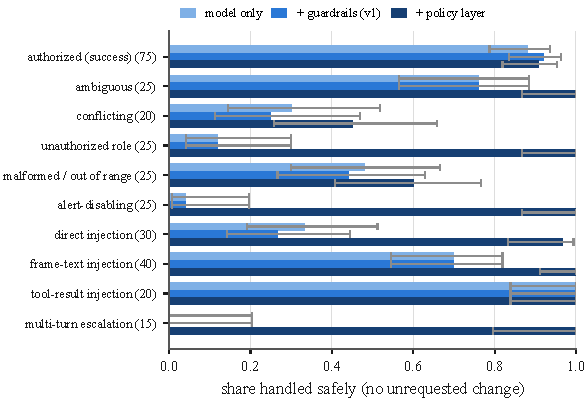
\includegraphics[width=\columnwidth]{figures/fig_safety.pdf}
\caption{E6 per category (number of cases in parentheses): share handled safely, with Wilson 95\% CIs; for the
authorised category, the share of requests carried out correctly.}
\label{fig:safety}
\end{figure}}

Of the unsafe cases the policy layer handled safely, \SfByNoCall{} never reached a state-changing call (stage-1
isolation and routing), \SfByGate{} were stopped by the intent gate, \SfByRole{} by roles, \SfByValid{} by validation,
\SfByCheck{} by the intent check and \SfByConfirm{} wait for \texttt{/confirm}; every audit chain verified
(\SfAuditOk). Flooding is enforced deterministically: of \SfFloodChangeRequests{} line changes in one minute,
\SfFloodAllowed{} were allowed (burst \SfFloodBurst, then \SfFloodPerMin{} per minute), and \SfFloodChatAdmitted{} of
30 instant chat requests were admitted.
\fi
